\chapter{Literature Review}
\label{ch:LR}
\section{Taxonomy for Intrusion Detection Systems}

\paragraph{}
In \cite{ids_taxonomy}, an attempt has been made to standardize a terminology for IDSs. Many different types of common in use IDSs are introduced in the paper, along with some upcoming possibilities.

\paragraph{}
Broadly, IDSs have been classified on the basis of 5 different features (Figure \ref{types_of_ids}).
\begin{figure}[h]
    \hfill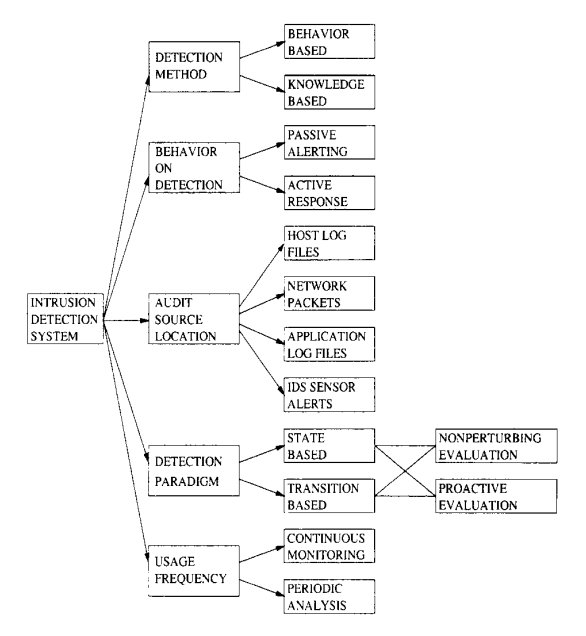
\includegraphics[width=0.8\textwidth]{Chapter2/types_of_ids}\hspace*{\fill}
    \caption{Types of IDS as mentioned in \cite{ids_taxonomy}}
    \label{types_of_ids}
\end{figure}
\begin{enumerate}
    \item On the basis of detection method:
        \begin{itemize}
            \item Behavior based
            \item Knowledge based
        \end{itemize}
    \item On the basis of behavior on detection:
        \begin{itemize}
            \item Passive filtering
            \item Active filtering
        \end{itemize}
    \item On the basis of audit source location:
        \begin{itemize}
            \item Host log files
            \item Network packets
            \item Application log files
            \item IDS sensor alerts
        \end{itemize}
    \item On the basis of detection paradigm:
        \begin{itemize}
            \item State based
            \item Transition based
        \end{itemize}
    \item On the basis of usage frequency:
        \begin{itemize}
            \item Continuous monitoring
            \item Periodic analysis
        \end{itemize}
\end{enumerate}

\paragraph{}
This work focuses only on behavior based IDSs. Various methods have been proposed using all kinds of machine learning models, some of which have been tested and compared in this work.

\section{Datasets}

\paragraph{}
When it comes to training and testing IDSs, the KDD'99 \cite{kdd99} and UNSW-NB15 \cite{unsw15} datasets are usually considered.
\begin{itemize}
    \item \textbf{KDD'99}: The KDD'99 dataset was curated in 1999 and was used for The Third International Knowledge Discovery and Data Mining Tools Competition 1999. It holds its popularity till date for training and testing models based on data mining and machine learning algorithms for extracting information out of network packet data. The dataset contained 41 features along with a label mentioning the type of attack detected. The dataset is a raw dump of network traffic, and barely processed for use in machine learning.
    \item \textbf{UNSW-NB15}: The UNSW-NB15 dataset was generated in 2015, and similar to KDD'99, is a dump of network traffic. However, it has been proccessed to fix the problems of KDD'99 \cite{unsw_comparison}. The dataset has a total of 49 features, including 2 class labels and over 2 million records. Since the dataset was generated more recently (2015), it is a more accurate example of network data traffic that an IDS might face in the current times. The class labels have classified 9 different kinds of attacks, some of which were not present in the KDD'99 dataset.
\end{itemize}

\paragraph{}
The UNSW-NB15 seemed to be a better dataset to use of this work, owing to its novelty and problems in KDD'99 that it addresses \cite{unsw_comparison}.

\section{UNSW-NB15}

\paragraph{}
The UNSW-NB15 dataset was released in 2015. It was generated using tcpdump tool to capture about 100GB of raw data. It has the following 9 types of attacks:
\begin{enumerate}
    \item Fuzzers: Fuzzing, or Fuzz Testing is a black box testing technique which aims at finding implementation bugs by injecting malformed or semi-malformed data in an automated fashion. Potential attackers may run fuzz tests on the network to find vulnerabilities that can be exploited.
    \item Analysis: Traffic analysis is a special type of inference attack technique that looks at communication patterns between entities in a system. Knowing who's talking to whom, when, and for how long, can sometimes clue an attacker in to information of which you'd rather she not be aware.
    \item Backdoor: A backdoor is a malware type that negates normal authentication procedures to access a system.\\
    Webserver backdoors are used for a number of malicious activities, including:
    \begin{itemize}
        \item Data theft
        \item Website defacing
        \item Server hijacking
        \item The launching of distributed denial of service (DDoS) attacks
        \item Infecting website visitors (watering hole attacks)
        \item Advanced persistent threat (APT) assaults
    \end{itemize}
    \item DoS: Denial of Service (DoS) is an attack which aims to make a host machine unavailable to its intended users by temporarily or indefinitely disrupting the host machines connection to the internet. \\
    Broadly, DoS attacks can be classified into 3 types:
    \begin{itemize}
        \item Volume Based Attacks: Includes UDP floods, ICMP floods, and other spoofed-packet floods. The attack’s goal is to saturate the bandwidth of the attacked site, and magnitude is measured in bits per second (Bps).
        \item Protocol Attacks: Includes SYN floods, fragmented packet attacks, Ping of Death, Smurf DDoS and more. This type of attack consumes actual server resources, or those of intermediate communication equipment, such as firewalls and load balancers, and is measured in packets per second (Pps).
        \item Application Layer Attacks: Includes low-and-slow attacks, GET/POST floods, attacks that target Apache, Windows or OpenBSD vulnerabilities and more. Comprised of seemingly legitimate and innocent requests, the goal of these attacks is to crash the web server, and the magnitude is measured in Requests per second (Rps).
    \end{itemize}
    \item Exploit: An exploit is a piece of software, a chunk of data, or a sequence of commands that takes advantage of a bug or vulnerability to cause unintended or unanticipated behavior to occur on computer software, hardware, or something electronic.
    \item Generic: This subset contains any general type of attack such as:
    \begin{itemize}
        \item Probe, which is a program or a device inserted into the network to monitor the network and collect data.
        \item User to Root Attacks (U2R), in which an attacker or a hacker tries to get the access rights from a normal host in order, for instance, to gain the root access to the system.
        \item Remote to Local Attacks (R2L), in which a remote user sends data packets to a machine over the internet, which he/she does not have the access to, in order to expose vulnerabilities and exploit privileges which a local user would have on the computer.
    \end{itemize}
    \item Reconnaissance: Active reconnaissance is a type of computer attack in which an intruder engages with the targeted system to gather information about vulnerabilities.
    \item Shellcode: A shellcode is a small piece of code used as the payload in the exploitation of a software vulnerability.
    \item Worm: A computer worm is a standalone malware computer program that replicates itself in order to spread to other computers. Often, it uses a computer network to spread itself, relying on security failures on the target computer to access it.
\end{enumerate}
\paragraph{}
The dataset contains 2,540,044 records with 49 features categorized into 6 categories.
\begin{enumerate}
\item \textbf{Flow Features:} \\
    1. srcip: Source IP address. \\
    2. sport: Source port number. \\
    3. dstip: Destinations IP address. \\
    4. dsport: Destination port number. \\
    5. proto: Protocol type, such as TCP, UDP.
\item \textbf{Basic Features:} \\
    6. state: The states and its dependent protocol e.g., CON. \\
    7. dur: Row total duration. \\
    8. sbytes: Source to destination bytes. \\
    9. dbytes: Destination to source bytes. \\
    10. sttl: Source to destination time to live. \\
    11. dttl: Destination to source time to live. \\
    12. sloss: Source packets retransmitted or dropped. \\
    13. dloss: Destination packets retransmitted or dropped. \\
    14. service: Such as http, ftp, smtp, ssh, dns and ftp-data. \\
    15. sload: Source bits per second. \\
    16. dload: Destination bits per second. \\
    17. spkts: Source to destination packet count. \\
    18. dpkts: Destination to source packet count.
\item \textbf{Content Features:} \\
    19. swin: Source TCP window advertisement value. \\
    20. dwin: Destination TCP window advertisement value. \\
    21. Stcpb: Source TCP base sequence number. \\
    22. dtcpb: Destination TCP base sequence number. \\
    23. smeansz: Mean of the packet size transmitted by the srcip. \\
    24. dmeansz: Mean of the packet size transmitted by the dstip. \\
    25. trans\_depth: The connection of http request/response transaction. \\
    26. res\_bdy\_len: The content size of the data transferred from http.
\item \textbf{Time Features:} \\
    27. sjit: Source jitter. \\
    28. djit: Destination jitter. \\
    29. stime: Row start time. \\
    30. ltime: Row last time. \\
    31. sintpkt: Source inter-packet arrival time. \\
    32. dintpkt: Destination inter-packet arrival time. \\
    33. tcprtt: Setup round-trip time, the sum of ’synack’ and ’ackdat’. \\
    34. synack: The time between the SYN and the SYN\_ACK packets. \\
    35. ackdat: The time between the SYN\_ACK and the ACK packets. \\
    36. is\_sm\_ips\_ports: If srcip (1) = dstip (3) and sport (2) = dsport (4), assign 1 else 0.
\item \textbf{Additional Generated Features:} \\
    37. ct\_state\_ttl: No. of each state (6) according to values of sttl (10) and dttl (11). \\
    38. ct\_flw\_http\_mthd: No. of methods such as Get and Post in http service. \\
    39. is\_ftp\_login: If the ftp session is accessed by user and password then 1 else 0. \\
    40. ct\_ftp\_cmd: No of flows that has a command in ftp session. \\
    41. ct\_srv\_src: No. of rows of the same service (14) and srcip (1) in 100 rows. \\
    42. ct\_srv\_dst: No. of rows of the same service (14) and dstip (3) in 100 rows. \\
    43. ct\_dst\_ltm: No. of rows of the same dstip (3) in 100 rows. \\
    44. ct\_src\_: ltm No. of rows of the srcip (1) in 100 rows. \\
    45. ct\_src\_dport\_ltm: No of rows of the same srcip (1) and the dsport (4) in 100 rows. \\
    46. ct\_dst\_sport\_ltm: No of rows of the same dstip (3) and the sport (2) in 100 rows. \\
    47. ct\_dst\_src\_ltm: No of rows of the same srcip (1) and the dstip (3) in 100 records.
\item \textbf{Labeled Features:} \\
    48. attack\_cat: The name of each attack category. \\
    49. label: 0 for normal and 1 for attack records.
\end{enumerate}

\section{Algorithms Used}

\paragraph{K-Nearest Neighbors} is an algorithm used for classification or regression. It takes the features and labels as inputs to train the model. Once trained, the classification is done on the basis of a majority vote. An object is classified as the class of the majority vote from the nearest \textit{k} vectors in the feature space. The parameter \textit{k} must be adjusted to specific use case scenarios. KNN is implemented in the scikit-learn library \cite{scikit-learn} as sklearn.neighbors.KNeighborsClassifier.

\paragraph{Naive Bayes} algorithm builds a conditional probability model with the assumption that all features are independent and have no correlation. Despite this, rather unrealistic assumption and seemingly oversimplified design, studies have shown that the algorithm is quite optimal \cite{nb_optimal}.

\paragraph{Decision Tree} is a method that generates tree-like model of decisions and their consequences. Various metrics, such as information gain, gini impurity etc. are used to decide which feature to split at every level in the tree. Scikit-learn library \cite{scikit-learn} implements decision tree in the class sklearn.tree.DecisionTreeClassifier. The choice of the metric to split the tree is given as a parameter in the class constructor.

\paragraph{Random Forest} \cite{random_forest} is an ensemble method in which many small decision trees are created at training time, and classification is done on the basis of a majority vote among the individual trees to decide on an object. This method addresses the issue of over-fitting in decision trees.

\paragraph{Extra Trees} is another ensemble method very similar to Random Forests. Studies suggest \cite{extra_tree} that Extra Trees tend to perform a bit worse when there is a high number of noisy features.
